\paragraph{}

In this section, we will explore three image processing applications: denoising, sharpening and image segmentation.
For each, we present a classic algorithm, a spectral approach to it and a comparison of them.
Finally, we present what has been done for 3D image processing using spectral graph theory, essentially using the graph laplacian operator.

\subsection{Denoising}

\paragraph{Background}

Even with high quality cameras, denoising and improving a taken picture remains important.
The two main issues that have to be addressed by denoising are blur and noise.
The effect of blur is internal to cameras since the number of samples of the continuous signal is limited and it has to hold the Shannon-Nyquist theorem \cite{buades_review_2005}.
Noise comes from the light aquisition system that fluctuates in relation to the amount of incoming photons.

To model these problems, we can formulate the deficient image as,
\[y = z + e,\]
where \(e\) is the noise vector of variance \(\sigma^2\), \(z\) the clean signal vector and \(y\) the noisy picture.

What we want is a high-performance denoiser, capable of scaling up in relation to increasing the image size and keeping reasonable performances.
The output image should come as close as possible to the clean image.
As an important matter, it is now accepted that images contain a lot of redundancy.
This means that, in a natural image, every small enough window has many similar windows in the same image.

\paragraph{Traditional, patch-based methods}

The image denoising algorithms review proposed by \cite{buades_review_2005} suggests that the NL-means algorithm, compared to other reviewed methods, comes closest to the original image when applied to a noisy image.
This algorithm takes advantage of the redundancy of natural images and for a given pixel i, predicts its value by using the pixels in its neighbourhood.

In \cite{dabov_image_2007}, the authors propose the BM3D algorithm, a denoising strategy based on grouping similar 2D fragments of the image into 3D data arrays. Then, collaborative filtering is performed on these groups and return 2D estimates of all grouped blocks.
This algorithm exposed state-of-the-art performance in terms of denoising at that time.
The results are still one of the best for a reasonable computational cost.

\paragraph{Global filter}

In the last couple of years, global image denoising filters came up, based on spectral decompositions \cite{glide_2014}.
This approach considers the image as a complete graph, where the filter value of each pixel is approximated by all pixels in the image.
We define the approximated clean image \(\hat{z}\) by,
\[\hat{z} = Wy,\]
where \(W\) is our data-dependent global filter, a \(n \times n\) matrix, \(n\) the number of pixels in the picture.
\(W\) is computed from the graph affinity matrix\footnote{Also called kernel matrix or similarity matrix} \(K\), also of size \(n \times n\), such as
\[K = {\mathcal{K}_{ij}},\]
where \(\mathcal{K}\) is a similarity function between two pixels \(i\) and \(j\).
As the size of \(K\) can grow very large, we sample the image and compute an approximated \(\hat{K}\) on this subset using the Nystr\"om extension.
\(K\) can in fact be approximated through its eigenvalues and eigenvectors.
Knowing that the eigenvalues of \(K\) decay very fast \cite{siam_slides_2016}, the first eigenvectors of the subset of pixels are enough to compute the approximated \(\hat{K}\).

Generally, as proposed in \cite{glide_2014} and \cite{talebi_asymptotic_2016}, to improve the denoising performance of global filters, pre-filtering techniques are used.
It is proposed to first apply a NL-means algorithm to the image to reduce the noise, but to still compute the global filter on the noisy input and apply the filter to the pre-filtered image.

\paragraph{Comparison between patch-based and global methods}

As \cite{talebi_asymptotic_2016} suggests, global filter methods have the possibility to converge to a perfect reconstruction of the clean image, which seems to be impossible for techniques like BM3D.
Global filtering also seems promising for creating more practical image processing algorithms.

The thesis \cite{kheradmand_graph-based_2016} proposes a normalised iterative denoising algorithm which is patch-based.
The work reports that this technique has slightly better results than the global filter but essentially has a better runtime performance.

\subsection{Sharpening}

\paragraph{Background}

Sharpening consists basically in a high-pass filter which will magnify high frequency details \cite{kheradmand_graph-based_2016}.
The two main issues again with this approach are that noise often displays high frequency attributes, which will be amplified by the filter.
Secondly, the phenomenon of overshooting and undershooting, which appears when sharpening already sharp parts (edges for example), will exhibit unpleasant artifacts.

Modeling the problem is the same as for denoising, \(\hat{z} = Fy\), \(F\) being our filter.

\paragraph{Classical Difference of Gaussian (DoG) operator}

This technique consists of computing the difference between two gaussian kernels, which will produce a range of different kernels with various frequencies.
Indeed, DoG involves subtracting a blurred version of the input image to another, less blurred version of this original image \cite{wiki:Difference_of_Gaussians}.
A blurred image can be obtained by convolving the input image with a gaussian kernel.
This gaussian blurring actually removes high-frequency spatial information.
So the idea is that by substracting this blurred image from a less blurred one, we will keep the high-frequency information, like a high-pass filter\footnote{More precisely, like a band-pass filter here}, which results in image sharpening.

\paragraph{Structure-aware sharpening}

We know from its definition \cite{kheradmand_non-linear_2015} that the smoothing filter \(W\) is a symmetric and doubly stochastic matrix\footnote{Depending on the used Laplacian definition. For example the one obtained by ``Sinkhorn" iterations \cite{milanfar_symmetrizing_2013}}.
So the largest eigenvalue \(\lambda_1 = 1\) shows that it has low pass filter characteristics.
With the definition of the Laplacian, in relation to the matrix \(W\) such as \(\Lapl = I - W\), we can consider that it is a data-adaptive high-pass filter \cite{kheradmand_graph-based_2016}.
So we can define a data-adaptive unsharp mask filter as
\[F_1 = I + \beta (I-W),\]
with \(\beta > 0\). This is basically a weighted high-pass filtered version of the input image \cite{siam_slides_2016}.

But with this approach, the noise amplifying and overshoot problems remain.
The proposed solution in \cite{kheradmand_non-linear_2015} applies first a smoothing filter to the image, then the unsharp mask filter and finally the same smoothing filter again.
The smoothing and sharping filters use possibly two different kernels matrices as basis.
The first smoothing filter aims to reduce the noise, while we still avoid over-smoothing.
The second and final smoothing controls the effect of the amplified noise and the overshoot artifacts.
This gives us the filter
\[F = W_1(I + \beta (I - W_2))W_1,\]
where \(W_1\) and \(W_2\) are constructed from the affinity matrices \(K_1\) and \(K_2\), which can differ in relation to the parameters of their respective kernel function.

\paragraph{Comparison}

As \cite{kheradmand_non-linear_2015} suggests, the structure-aware sharpening is data-adaptive and more noise robust than a classical DoG filter.
Even though, both approaches use a similar concept.
The proposed filter is actually a data-derived DoG-based filter.
We can rewrite the proposed filter as
\[F = (1+\beta) W_1^2 - \beta W_1 W_2 W_1,\]
where we can actually see the difference between two versions of the input image.

\subsection{Image Segmentation}

\paragraph{Background}

To recognise patterns, find groups and cut images is a similar problem to graph partitioning.
As is it known, most formulations of partitioning a graph result in a NP-hard problem.
So it will be our goal to approximate quickly good partitions instead of looking for an optimal solution.

A graph \(G = (V, E)\) is partitioned into two disjoint sets \(A\) and \(B\) such as \(A \cup B = V\) and \(A \cap B = \emptyset\) by removing edges between \(A\) and \(B\).
One can compute the value of such a \(cut\) with the degree of dissimilarity between \(A\) and \(B\), which is calculated from the total weight of the removed edges:
\[cut(A, B) = \sum_{u\in A, v\in B} w(u, v).\]

\paragraph{\textit{Minimum cut}}

The most common way of partitioning a graph is the \textit{minimum cut}.
This problem consists in looking for the optimal bipartition of a graph, which is one that minimises the \(cut\) value.
The \textit{minimum cut} problem is well-studied and has efficient algorithms for solving it, even though it has an exponential amount of partitions that can be explored.

Some work on image segmentation using the \textit{minimum cut} has been done \cite{wu_optimal_1993} \cite{estrada_spectral_2004} \cite{felzenszwalb_efficient_2004}.
But the results can only be qualified as proposals for recognised regions, such does \cite{estrada_spectral_2004} and would need further optimisation to be the final groups.
For instance, \cite{wu_optimal_1993} introduced a cut criterion using \textit{minimum cut} on a graph but it was observed that it favors finding too small components and \cite{felzenszwalb_efficient_2004} tries to optimise the latter.

However, this problem still remains and \textit{minimum cut} can produce bad groups on certain cases.
Additionnaly, these cases often appear in natural images, where it is more important to group a large area of the background before small details.

\begin{figure}[!htbp]
 \centering
  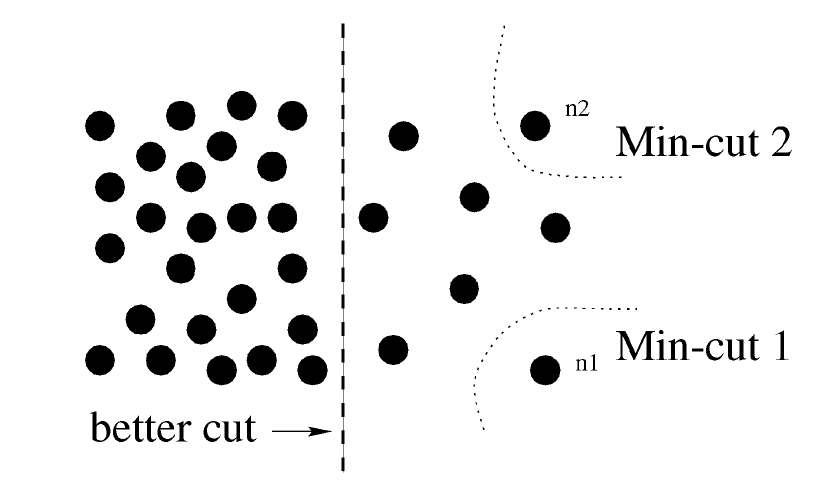
\includegraphics[width=\textwidth]{img/mincutproblem.png}
 \caption{Bad partitioning from \textit{minimum cut} in a particular case \cite{shi_normalized_2000}}
\end{figure}

\paragraph{\textit{Normalised cut}}

To improve this state, \cite{shi_normalized_2000} proposed, instead of looking at the total weigh of the edges connecting two groups, to look at a fraction of the total edge connections to all nodes.
This is the \textit{normalised cut}, or \(Ncut\).
The disassociation measure can be formulated as:
\[Ncut(A, B) = \frac{cut(A, B)}{assoc(A, V)} + \frac{cut(A, B)}{assoc(B, V)},\]
where \(assoc(A, V) = \sum_{u\in A, t\in V} w(u, t)\), the total connection from the nodes in A to all nodes in the graph.

The goal is still to minimise the \(Ncut\) value, but when \(cut\) is small for isolated pixels, the fraction will be greater because the similarity \(assoc\) between this one pixel and all pixels will be small.
This fraction's denominator will be bigger if the similarity between the selected pixels and all pixels is more important, which makes the fraction smaller.

As it follows, we can define the normalised association measure within groups, such as
\[Nassoc(A, B) = \frac{assoc(A, A)}{assoc(A,V)} + \frac{assoc(B, B)}{assoc(B, V)},\]
where \(assoc(A, A)\) is the total weights of edges inside group \(A\).
This measure quantifies how tightly the nodes of a group are connected to each other.
Deriving the \(Ncut\) equation, we can define that
\[Ncut(A, B) = 2 - Nassoc(A, B).\]

It was shown by \cite{papadimitriou_npcompleteness_1997} and \cite{shi_normalized_2000} that minimising the \(Ncut\) exactly is a NP-complete problem.
However, \cite{shi_normalized_2000} proposes a method to appoximate discrete solutions efficiently for the \textit{normalised cut} problem.

Indeed, the proposed algorithm starts by computing the associated similarities for graph \(G = (V, E)\) for the image and store it in the matrices \(K\) and \(D\).

Then, solve \((D-K)x = \lambda Dx\) for the eigenvectors with the smallest eigenvalues.
The way this equation is derived is explicitly shown in \cite{shi_normalized_2000}.
The eigenvector with the second smallest is used to bipartition the graph by finding the best splitting point to minimise \(Ncut\).
After that, it is possible to use the other eigenvectors to bipartition the graph even more.
Once this is done, we can recursively apply the same algorithm on the segmented groups, stoping when the maximum number of groups is reached or the partitions are not good enough depending on an empirical threshold.

\paragraph{Edge separators and spectral rounding}

Introduced by \cite{tolliver_graph_2006}, edge separators of a graph are created by iteratively reweighting edges until the graph disconnects into a certain number of groups.
At each iteration, only a small number of eigenvectors are computed to reweight the edges.
This spectral rounding method produces directly discrete solutions, and seems to compare nicely against the \(Ncut\) approximation by producing more human-like results \cite{tolliver_spectral_2006}.

\subsection{3D spectral image processing}

In general, \cite{zhang_spectral_2010} sets a very good overview of most variants and applications of spectral processing.
